\documentclass[]{thesis-ekf}
\usepackage[T1]{fontenc}
\PassOptionsToPackage{defaults=hu-min}{magyar.ldf}
\usepackage{fancyvrb,listingsutf8,xcolor,caption,graphicx}
\usepackage{amsthm,amsmath,amssymb,listings}
\usepackage[magyar]{babel}
\lstset{
	inputencoding=utf8/latin2,
	language=Java,
	basicstyle=\footnotesize,
	numbers=left,
	breaklines,
	postbreak=\hbox{$\color{red}\hookrightarrow\ $},
	xleftmargin=2cm,
	xrightmargin=2cm,
	backgroundcolor=\color{gray!30},
	frame=tlbr,
	framesep=3pt,
	keywordstyle=\bfseries\color{blue},
	commentstyle=\itshape\color{teal}
}
\theoremstyle{definition}
\newtheorem{definicio}{Definíció}[chapter]
\DeclareMathOperator{\tg}{tg}
\setlength{\headheight}{15pt}
\renewcommand{\lstlistingname}{kód}

\begin{document}
\institute{Informatikai Kar -- IK}
\title{Arduino robotfejlesztés android alkalmazás használatával}
\author{Bozó Tamás Dániel\\Programtervező informatikus BSc}
\supervisor{Balla Tamás\\Tanársegéd}
\city{Eger}
\date{2021}
\maketitle
\tableofcontents
\chapter*{Bevezetés}
\begin{flushright}
	\emph{,,There are an endless number of things to discover about robotics. A lot of it is just too fantastic for people to believe.'' -- Daniel H. Wilson}
\end{flushright}

A mai világban egyre több helyen alkalmaznak robotokat. Akár a munkahelyen a termelés felgyorsítására, az egészségügyben az orvosok segítésére, vagy csak az otthonunkban különböző feladatok elvégzésére. Azért választottam ezt a témát diplomamunkám elkészítéséhez, ugyanis az egyetemi tanulmányaim befejezése utáni célom általános iskolai tanárként elhelyezkedni lakóhelyemen és a diákok ismereteit az alaptanterven túl bővíteni a robotika világában.

Szakdolgozatom témája egy olyan robot építése és programozása, mely egy vonallal kirajzolt pályát képes követni, a pályán található esetleges akadályokat érzékelni és kikerülni, valamint egy olyan android rendszerrel rendelkező készülékre telepíthető applikáció fejlesztése melynek segítségével a felhasználó is képes irányítani. A robot megtervezése során igyekeztem egy olyan felépítésre törekedni, amit otthon hobbi felhasználók, de akár általános iskolások is képesek megépíteni, valamint egy olyan programkód írására, amit könnyen meg lehet érteni és esetleg változtatni/bővíteni.

A telefonos applikáció megvalósítására egy olyan kezelőfelületet akartam létrehozni, mely egyaránt biztosítja a lehetőséget a valós idejű irányításra, valamint a robot működésének monitorozására is.

Programozási nyelvként a C++-t és a Java-t választottam. A Java egy széles körben elterjedt nyelv, melyet könnyen lehet értelmezni, a C++ pedig az Arduino által támogatott nyelv, fejlesztői környezetnek pedig az Arduino IDE és Android Studio nevű alkalmazásokat használtam.

A dokumentumban olvashatunk a diplomamunkám elkészítéséhez választott technológiákról és programozási nyelvekről \az{\ref{fejezet_1}.}~fejezetben, a téma választása után kitűzött célokról és követelményekről \az{\ref{fejezet_2}.}~fejezetben, a fejlesztés és tesztelés során használt hardverekről \az{\ref{fejezet_3}.}~fejezetben, az Android applikáció felületterveiről és a robot belső állapotairól, valamint ezek működéséről \az{\ref{fejezet_4}. és \ref{fejezet_5}.}~fejezetekben, a fejlesztés során szerzett személyes tapasztalataimról \az{\ref{fejezet_6}.}~fejezetben. A \ref{fejezet_7}. és \ref{fejezet_8}.~fejezetekben pedig a projekt összeállításához tartózó útmutatóról és a továbbfejlesztési lehetőségekről.
\chapter{Arduino és Android bemutatása}\label{fejezet_1}
\emph{,,Programming today is a race between software engineers striving to build bigger and better idiot-proof programs, and the Universe trying to produce bigger and better idiots. So far, the Universe is winning'' -- Rick Cook, The Wizardry Compiled}
\section{Az Arduino}
Az Arduino\cite{Arduino} egy szabad szoftveres, nyílt forráskódú elektronikai fejlesztőplatform. Széles tömegek számára elérhető, mivel olcsó, könnyen beszerezhető, egyszerűen programozható és csatlakoztatható más eszközökhöz. A fejlesztői platform az úgynevezett "IDE"-ből és egy Arduino Board-ból áll. Az előbbi segítségével programokat írhatunk és tesztelhetünk a számítógépen, utóbbi pedig egy hardver eszköz, amelyre az elkészített programokat feltölthetjük a számítógépen keresztül, majd az eszközöket vezérelhetjük a segítségével.

Az Arduino lap kereskedelmi forgalomban kapható, előre összeszerelt, vagy otthon összeszerelhető alkatrészcsomagként. Mivel nyílt forráskódú a hardver is, bárki készíthet magának saját változatot belőle, vagy az eredetivel kompatibilis klónt.
\subsection{A fejlesztéshez választott alaplap}\label{arduino_alaplap}
A fejlesztés megkezdése előtt szükséges volt kiválasztanom azon hardverelemeket, melyek a robot mozgását, és vezérlését biztosítják, ezek:
\begin{itemize}
	\item 4 db villanymotor
	\item 2 db HW-201 típusú infravörös szenzor
	\item 1 db HC-SR04 típusú ultrahang szenzor
	\item 1 db HC-05 típusú Bluetooth modul
	\item 1 db SG90 típusú szervo motor
	\item 1 db Adafruit Motorvezérlő Shield
\end{itemize}

Miután a hardverelemeket kiválasztottam, szükségem volt egy alaplapra is, mely a robot központi része lesz. A választásom az Arduino UNO-ra esett, mivel ez rendelkezik megfelelő számú be- és kimenettel, valamint a motorok vezérléséhez használt shield-el is kompatibilis.

Az UNO egy ATmega328P mikrokontrollerrel van felszerelve, valamint 32 KB Flash memóriával rendelkezik, melyben a feltöltött program tárolódik. Csatlakozók szempontjából 6db analóg és 14db digitális tüske, valamint egy USB port található rajta (a kiosztást az \ref{uno_pins}~ábrán láthatjuk).
\begin{figure}[h]
	\centering
	\includegraphics[width=\linewidth]{images/arduino/Uno_Pins}
	\caption{Az UNO tüskekiosztása}
	\label{uno_pins}
\end{figure}
\subsection{Az IDE felépítése és használata}\label{arduino-IDE}
A programok írását és alaplapra való feltöltését az Arduino IDE segítségével tehetjük meg (\ref{IDE_felépítés}~ábra), mely egy felhasználóbarát fejlesztőkörnyezet.

Használatakor láthatjuk a használt USB port sorszámát és az ehhez csatlakoztatott alaplat típusát, továbbá a programunk nevét is.

A szerkesztőfelületen írhatjuk a programot és az alatta található üzenetfelületen kap a felhasználó visszajelzést arról, hogy a program feltöltése sikeres volt-e, illetve az előforduló problémákról is.

A program feltöltésén kívül lehetőségünk van az ellenőrzésre is, továbbá az eszköztárban található menüpontok segítségével megnyithatjuk a soros monitort, létrehozhatunk új projektet, de akár a használt alaplap és USB port is megváltoztatható, így egyszerre akár több alaplapot is csatlakoztathatunk a számítógéphez.
\begin{figure}[h]
	\centering
	\includegraphics[width=\linewidth]{images/arduino/IDE_felépítés}
	\caption{Az IDE felülete}
	\label{IDE_felépítés}
\end{figure}

Az IDE teljes felépítése megtekinthető az Arduino hivatalos honlapján\cite{Arduino IDE}.
\subsection{A C++ nyelv}
A C++\cite{CPP} egy általános célú, magas szintű programozási nyelv. Támogatja a procedurális, az objektumorientált és a generikus programozást, valamint az adatabsztrakciót. Napjainkban szinte minden operációs rendszer alá létezik C++ fordító.

A nyelv a C programozási nyelv hatékonyságának megőrzése mellett törekszik a könnyebben megírható, karbantartható és újrahasznosítható kód írására, ez azonban sok kompromisszummal jár. Erre utal, hogy általánosan elterjedt a mid-level minősítése is, bár szigorú értelemben véve egyértelműen magas szintű.

Bjarne Stroustrup kezdte el a C++ programozási nyelv fejlesztését a C programozási nyelv kiterjesztéseként, más nyelvekből véve át megoldásokat (Simula67, Algol68), ötleteket (ADA).

A nyelv első, nem kísérleti körülmények közt való használatára 1983-ban került sor, 1987-ben pedig nyilvánvalóvá vált, hogy a C++ szabványosítása elkerülhetetlen. Ez a folyamat 1991 júniusában kezdődött el, amikor az ISO szabványosítási kezdeményezés részévé vált.

A C++ programozási nyelv szabványát 1998-ban hagyták jóvá ISO/IEC 14882:1998 néven, az aktuális, 2017-es változat kódjelzése ISO/IEC 14882:2017.
\section{A Java nyelv és az Android}
A Java\cite{Java} általános célú, objektumorientált programozási nyelv, amelyet a Sun Microsystems fejlesztett a ’90-es évek elejétől kezdve egészen 2009-ig, amikor a céget felvásárolta az Oracle. 2011-ben a Java 1.7-es verzióját az új tulajdonos gondozásában adták ki.

A Java alkalmazásokat jellemzően bájtkód formátumra alakítják, de közvetlenül natív (gépi) kód is készíthető Java forráskódból. A bájtkód futtatása a Java virtuális géppel történik, ami vagy interpretálja a bájtkódot, vagy natív gépi kódot készít belőle, és azt futtatja az adott operációs rendszeren. Létezik közvetlenül Java bájtkódot futtató hardver is, az úgynevezett Java processzor.

A Java nyelv a szintaxisát főleg a C és a C++ nyelvektől örökölte, viszont sokkal egyszerűbb objektummodellel rendelkezik, mint a C++.
\subsection{Miért pont Android?}
A modern világban szinte minden ember rendelkezik, vagy találkozott már olyan telefonnal, mely valamilyen mobil OS-t\footnote{mobil operációs rendszer} futtat, melyek közül a legjobban elterjedt az Android\cite{Android} és az iOS.

Az Android-ot kezdetben az Android Inc. fejlesztette, azonban 2005-ben a Google felvásárolta és a fejlesztést az Open Handset Alliance folytatta, melyet ~82 cég alkot, köztük az Intel, a HTC, a Samsung és az eBay is.

Az Android-ot futtató telefonok a felhasználók számára nagy rendszer-testreszabási lehetőségeket nyújtanak, valamint széleskörű kompatibilitást különféle kiegészítőkkel, például vezeték nélküli eszközök, okos óra/tv.

Android-ra a fejlesztők Java vagy Kotlin programozási nyelv segítségével tudnak programokat írni, fejlesztőkörnyezetnek pedig legelterjedtebb az Android Studio, melyről a következő oldalon részletesen is olvashatunk.
\subsection{Az Android Studio felépítése és használata}\label{android-studio}
Az Android Studio\cite{Android} egy integrált fejlesztőkörnyezet (IDE) az Android platformra való fejlesztéshez. 2013. május 16-án jelentette be a Google I/O konferencián a Google termékmenedzsere Katherine Chou. Az Android Studio szabadon elérhető Apache License 2.0 alatt.

A JetBrains IntelliJ IDEA-ján alapuló szoftvert, az Android Studiot kifejezetten androidos fejlesztésre tervezték. Letölthető Windowsra, Mac OS X-re és Linuxra is egyaránt, és teljes egészében helyettesíti az Eclipse Android Development Tools (ADT)-ját. A Google elsődleges IDE-jének választott a natív Android alkalmazás fejlesztésre.
\begin{figure}[h]
	\centering
	\includegraphics[width=\linewidth]{images/android/android_ide}
	\caption{Az Android Studio}
	\label{android_ide}
\end{figure}

Az IDE használata hamar megtanulható, ugyanis felhasználóbarát felépítéssel rendelkezik(\ref{android_ide}~ábra). Az alkalmazás dizájnjának megalkotására egy beépített felületet biztosít az Android Studio, ami WYSIWYG\footnote{What you see is what you get/Azt kapod, amit látsz} alapon működik.

Az IDE tartalmaz továbbá egy beépített navigációs felületet, ahol a felhasználó a megnyitott projekt elemeit találja meg. A projektben megtalálható fájlok mappaszerkezetét látja a felhasználó, így a dizájnért felelős .xml kiterjesztésű fájlok a 'res/layout' mappában találhatóak és az ugyanazon képernyőhöz tartozó fekvő és álló elrendezés pedig a képernyő mappájában.

A navigációs sávon kívül a felhasználó több, a projekt állapotához tartozó információt is kap, mint például a projekt futtatásakor az ablak alján megjelenő Event Log, ami a programmal kapcsolatban ad visszajelzést (pl: sikeres volt-e a build), vagy az eszköztár alatt látható a készülék, vagy AVD\footnote{Android Virtual Device} neve, amelyen a program futtatása fog történni.

További hasznos tulajdonság, hogy amennyiben a fejlesztő hibát követ el a forráskód írása közben az IDE figyelmeztet erről, valamint az ebből eredő összes hibát megjelöli és a hiba megoldására is tanácsot ad a felhasználónak (\ref{ide_hiba}~ábra), valamint a projektben történő refaktorálást is könnyen megtehetjük a Shift+F6 billentyűkombinációval, aminek hatására az IDE nem csak az adott sorban, hanem minden használati esetnél is módosítja az általunk kijelölt objektumot.
\begin{figure}[h]
	\centering
	\includegraphics[width=\linewidth]{images/android/ide_hibaérzékelés}
	\caption{Hiba jelzése az IDE-ben}
	\label{ide_hiba}
\end{figure}

\chapter{Követelményspecifikáció}\label{fejezet_2}
Ebben a fejezetben arról fogok beszámolni, hogy a projekt kigondolásakor, milyen célt tűztem ki magamnak, valamint ennek megvalósítására milyen komponenseket használtam.
\section{Vágyálomrendszer leírása}\label{vágyálom}
A projekt megalkotásakor a célom egy olyan robot kifejlesztése volt, amely képes egy megadott pályát követni, a követés közben észlelt bármekkora méretű akadályt kikerül és ezután a követendő pályát újra megtalálni, valamint egy olyan telefonos alkalmazást kifejleszteni, mellyel a robotot irányítani tudjuk, a robot által vezetett napló tartalmának megtekintését lehetővé teszi, valamint a naplót a készülékre lehessen menteni.

Szerettem volna ezeket úgy megvalósítani, hogy a végtermékkel különböző életkorú diákok oktatását lehessen segíteni, de otthoni felhasználáshoz is szórakoztató időtöltés legyen akár egyszerre több embernek is.

A 2020-as Nemzeti Alaptantervben\cite{NAT} az általános iskolás diákok számára a Digitális Kultúra tárgy magába foglalja a robotika oktatását 5. és 6. osztályban 11 óra alkalmával, valamint 7-8. osztályosoknak 8 órában. Az órák alatt a diákok számára a javasolt tevékenység különböző programok megírása blokkprogramozással, ezért nekik lehetőséget akarok biztosítani egy másik programozási módszer megismerésére.

Középiskolások részére a tárgyban megtalálható a Mobiltechnológiai ismeretek témakör, melyet 9. és 11. osztályban 4-4 órában tanulnak a diákok. Az ő részükre a telefonra fejlesztett applikációval szeretnék egy példát mutatni a mobiltechnológiai eszközök segítségével megvalósított együttműködésre.

Hobbifelhasználóknak pedig egy olyan kikapcsolódási lehetőséget akartam biztosítani, mellyel maguk építhetnek meg egy olyan robotot, amit utána irányítani is tudnak.
\section{Követelmények}\label{követelmény}
Miután kitűztem a célt, amit el szeretnék érni meg kellett fogalmaznom néhány elvárást is.

\textbf{A kód könnyen módosítható legyen.} Ahhoz, hogy az általános iskolai diákok számára ne legyen bonyolult a projekt, szükséges, hogy az alapoktól kezdve tudjuk megmutatni nekik hogyan is épül fel.

\textbf{A projekt legyen érdekes.} A diákok számára egy olyan példát kell biztosítani, mely felkelti az érdeklődésüket.

\textbf{Sokoldalú felhasználás.} Mivel nem csak oktatási célra szánom a projektemet, szükségesnek tartottam, hogy a hétköznapi felhasználók is szórakoztatónak találják.
\section{Jelenlegi helyzet leírása}\label{jelenlegi_helyzet}
A projekt jelenlegi állapotában a \ref{vágyálom}.~fejezetben megfogalmazottaknak sikerült eleget tennem. A robot az alváz elején található infravörös szenzorok segítségével képes követni egy előre megadott pályát, ezen a kanyarokat be tudja venni (az éles, ~45-90°-os kanyarok néha problémát okozhatnak), majd ugyanezen szenzoroknak köszönhetően egy akadály kikerülése után a követendő pályát képes ismételten megtalálni.

A felhasznált ultrahang szenzor biztosítja azt, hogy a robot nem fog akadálynak ütközni a pálya követése közben, a Bluetooth modulnak köszönhetően pedig a telefonos applikációval rá tudunk csatlakozni a robotra.

A telefonos applikációban a robot vezérlésének több részét is el tudjuk végezni. Először is el tudjuk dönteni, hogy a robot kövesse-e a pályát vagy mi magunk szeretnénk irányítani. Másodszor a robot irányításakor mi tudjuk megmondani az irányt, amerre szeretnénk, ha a robot mozogna. Harmadszor pedig a robot által létrehozott naplófájlt meg tudjuk a telefonon tekinteni, a telefonra le tudjuk menteni, vagy a robot memóriájából ki tudjuk törölni.
\chapter{Funkcionális specifikáció}\label{fejezet_3}
A fejezetben a projekt használati lehetőségeit mutatom, valamint \az{\ref{fejezet_2}.~fejezetben} megfogalmazottaknak feleltetem meg a termékemet, majd ismertetem a fejlesztéshez és teszteléshez használt hardverelemek néhány tulajdonságát.
\section{Használati esetek}
A projektnek egy felhasználója van, egy személy. A felhasználó két különböző szoftverrel érintkezik és ezek más-más funkciókkal rendelkeznek.

A roboton futó szoftver képes a naplófájlhoz új eseményeket hozzáadni, eseményeket törölni, a naplófájlt a telefonra elküldeni, valamint képes a pálya követésére.

Az okostelefonon futó szoftver el tudja végezni a robot irányítását, a vonal követését szüneteltetheti/indíthatja el és a robot által készített naplófájl tartalmát lekérheti és mentheti.
\section{Követelmény megfeleltetés}
A következőkben részletezem, hogy a \ref{követelmény} pontban megfogalmazottaknak hogyan tettem eleget.
\subsection{Könnyű módosíthatóság}
Az Arduino alaplapon futó kódban minden olyan egységet, mely egy szenzorról beérkező értéket használ fel egy feltétel vizsgálatához, vagy változó értékének módosításához igyekeztem külön metódusba építeni, így a kód gyorsan és biztonságosan módosítható.

A módosíthatóságnak köszönhetően a diákok számára létre lehet hozni egy olyan struktúrát a projektben, melyben kezdetben csak az infravörös szenzorokat használjuk LED-el, majd lépésről-lépésre a LED-et lecseréljük a motorokra, valamint hozzáadjuk az ultrahang szenzort és végül ezeknek a működését hangoljuk össze.
\subsection{Érdekes projekt}
A projekt véleményem szerint a diákok számára kellő érdekességgel bír, ugyanis nem csak új ismeretet tudnak vele szerezni, hanem egy interaktív óra lehetőségét is magában hordozza.
\subsection{Sokoldalú felhasználás}
A projekt nem csak az irányítás és a pályakövetés lehetőségét biztosítja. Ha szeretnénk a robotnak egyre összetettebb és nehezebb pályákat tudunk építeni, emelkedőkkel, nagyobb akadályokkal összetettebb kanyarokkal, ezzel tesztelve, hogy mi az amire a robot képes és mire nem. Más lehetőség, hogy az otthoni felhasználás során a roboton található modulok, vagy a telefonos alkalmazás átalakításával a projekt továbbfejlesztésére is van lehetőség.
\section{A fejlesztéshez használt hardver}\label{telefonok}
Az \ref{arduino_alaplap}~fejezetben olvashattunk az alaplap adatairól, most bemutatom a további hardverelemeket, illetve a teszteléshez felhasznált telefonokat.

\textbf{A robothoz tartozó hardverelemek}
\begin{center}
	\begin{tabular}{|l|c|c|}
		\hline
		\multicolumn{1}{|c|}{\textbf{Megnevezés}}&\textbf{Csatlakozás}&\textbf{Működési feszültség}\\
		\hline
		Villanymotor&2 db digitális port/motor&3-6 Volt\\
		\hline
		SG90 szervo motor&1 db analóg port&4.8-6 Volt\\
		\hline
		HC-SR04 szenzor&2 db digitális port&5 Volt\\
		\hline
		HW-201 szenzor&1 db analóg port&5 Volt\\
		\hline
		HC-05 Bluetooth modul&2 db digitális port&3.3-5 Volt\\
		\hline
	\end{tabular}
\end{center}

\textbf{A telefonok adatai}
\begin{center}
	\begin{tabular}{|l|c|c|}
		\hline
		\multicolumn{1}{|c|}{\textbf{}}&\textbf{Samsung Galaxy A71}&\textbf{Alcatel Pop D1}\\
		\hline
		\textbf{Processzor}&Qualcomm Snapdragon 730&ARM Cortex-A7\\
		\hline
		\textbf{Processzormagok száma}&8&2\\
		\hline
		\textbf{Processzor sebessége}&2.2 GHz&1 GHz\\
		\hline
		\textbf{RAM mérete}&6 GB&512 MB\\
		\hline
		\textbf{Akkumulátor típusa}&Lithium-Polymer&Lithium-Ion\\
		\hline
		\textbf{Akkumulátor kapacitás}&4500 mAh&1300 mAh\\
		\hline
		\textbf{Android verzió}&10&4.4.2 KitKat\\
		\hline
		\textbf{Bluetooth verzió}&v5.00&v4.00\\
		\hline
	\end{tabular}
\end{center}
\chapter{Belső állapotok és felületterv}\label{fejezet_4}
\emph{,,Any fool can write code that a computer can understand. Good programmers write code that humans can understand.'' -- Martin Fowler}
\section{A robot belső állapotai}
A robot működése során többször is változik a belső állapota, a változást a telefonos applikációból kapott adat, valamint a roboton található szenzorok idézik elő.
\subsection{Kezdőállapot}\label{kezdokepernyo_allapot}
\begin{figure}[h]
	\centering
	\includegraphics[width=\columnwidth]{images/grafok/fomenu_graf}
	\caption{Fő állapotok közötti átmenet}
	\label{start_allapot}
\end{figure}
A robot indulását követően a kezdőállapotból minden alkalommal a telefonról kapott jel fogja kimozdítani. Amint van csatlakoztatott eszköz a robot elkezdi várni az utasítást. A telefonról érkező utasítás 3 számkód lehet. Minden számkód egy-egy folyamatért felel, mely lehet:
\begin{itemize}
	\item Irányítás folyamata = 111-es kód
	\item Pályakövetés folyamata = 222-es kód
	\item Naplózás folyamata = 333-as kód
\end{itemize}
\subsection{Az irányítás folyamata}\label{controlkepernyo_allapo}
Abban az esetben, ha az applikáció főmenüjében az ’irányítás’ lehetőséget választjuk a robot elkezd várni a bejövő utasításra. Amennyiben ez az utasítás megegyezik a folyamatot megszakító kóddal a robot visszatér a kezdőállapotába.

Ha a kapott utasításból származó kód az 'F', 'L', 'R', 'B', 'S' betűk valamelyike a robot az ehhez tartozó mozgást végzi el.
\begin{itemize}
	\item F = Előrehaladás
	\item L = Balkanyar
	\item R = Jobb kanyar
	\item B = Tolatás
	\item S = Állj
	\item T = Teszt folyamat
\end{itemize}

A telefon a kódot mindaddig küldi ki a robotnak, amíg az adott gomb lenyomva van. Amint a gombot felengedjük a telefon elküldi a robot megállítására szolgáló 'S' kódot.
\begin{figure}[h]
	\centering
	\includegraphics[width=\columnwidth]{images/grafok/iranyitas_graf}
	\caption{Bluetooth irányítás}
	\label{iranyitas_graf}
\end{figure}
\subsection{Automata követés folyamata}\label{followkepernyo_allapot}
Amennyiben a kezdőképernyőn a ’követés’ gombot nyomja meg a felhasználó a roboton található szenzorok végzik el a belső állapotok változtatását.
Ekkor a robot a váz elején található Infravörös szenzorok által érzékelt vonal követését hajtja végre és ebből az állapotából két esetben lép ki:
\begin{itemize}
	\item Valamelyik IR szenzor jelzést ad a vonal kanyarodásáról
	\item A robot elején található UH szenzor akadályt érzékel
\end{itemize}
\begin{figure}[h]
	\centering
	\includegraphics[width=\columnwidth]{images/grafok/kovetes_graf}
	\caption{A követés folyamata}
	\label{kovetes_graf}
\end{figure}

Mindaddig, míg a robot nem érzékel akadályt vagy kanyart a motorok egyforma sebességgel forognak előre. Amennyiben kanyarról ad jelzést valamely IR szenzor a robot korrigálást hajt végre a megfelelő motorok paramétereinek megváltoztatásával (nyomaték, irány). Amint a korrigálás megtörtént és a jelzést leadó szenzor visszaáll eredeti értékére, a robot visszatér a követő állapotba.

Amennyiben akadály érzékelése történik minden motor leállításra kerül, majd a robot elvégez egy pásztázást a váz elején található szervó motor és UH szenzor segítségével. A pásztázás befejezését követően az akadály megkerülése történik jobb vagy bal irányba, majd a pálya megtalálását követően a robot ismét követi azt (erről bővebben olvashatunk a \ref{180°-sonar}.~fejezetben).
\subsection{A naplózási folyamat}\label{naplokepernyo_allapot}
A naplózási folyamat során a robot nem végez mozgást, csak a telefonnal kommunikál és az onnan kapott kód alapján három feladatot tud elvégezni:
\begin{itemize}
	\item A folyamatból kilép, ha a bejövő kód 'B'
	\item A telefonra küldi a naplófájl jelenlegi tartalmát, ha a kód 'G'
	\item A naplófájl tartalmát üríti a memóriájából, ha a kód 'D'
\end{itemize}
\begin{figure}[h]
	\centering
	\includegraphics[width=\columnwidth]{images/grafok/log_graf}
	\caption{Naplózási állapotok}
	\label{log_graf}
\end{figure}
\section{Android képernyőtervek}
Az applikációnak négy képernyője van, ezek:
\begin{itemize}
	\item Kezdőképernyő
	\item Súgó képernyő
	\item Automata követés képernyő
	\item Bluetooth irányítás képernyő
	\item Naplózási képernyő
\end{itemize}

A képernyők között az alkalmazásban megtalálható gombok segítségével navigálhatunk.

\textbf{Kezdőképernyő:} Az alkalmazás elindításakor a felhasználót ez a képernyő üdvözli, ahol öt gomb közül választhatunk, melyek különböző funkciókért felelnek, ezek:
\begin{itemize}
	\item \underline{Eszközök:} A megnyomása után a képernyőn megjelenik a párosított Bluetooth-eszközök listája, melyből ki tudjuk választani a számunkra megfelelőt.
	\item \underline{Súgó:} Az applikációba beépített ’Súgó’ képernyő válik aktívvá ahol a felhasználó minden funkciót megismerhet.
	\item \underline{Követés:} Átirányítja a felhasználót az ’Automata követés’ képernyőjére.
	\item \underline{Irányítás:} A felhasználó a ’Bluetooth irányítás’ képernyőre kerül, ahol a robotot tudjuk vezérelni.
	\item \underline{Log:} A naplófájl megtekintésére és mentésére szolgáló képernyőre kerül a felhasználó.
\end{itemize}
\begin{figure}[h]
	\centering
	\includegraphics[width=\columnwidth]{images/app_screen/home_screen}
	\caption{Kezdőképernyő}
	\label{home-screen}
\end{figure}

\textbf{Súgó képernyő:} A képernyő tartalmazza a funkciók rövid leírását.
\begin{figure}[h]
	\centering
	\includegraphics[width=\columnwidth]{images/app_screen/help_screen}
	\caption{Súgó képernyő}
	\label{help-screen}
\end{figure}
\begin{itemize}
	\item \underline{Home ikon:} A kezdőlapra navigálja a felhasználót.
	\item \underline{Szöveg felület:} A kiválasztott gomb által tartalmazott leírást jeleníti meg.
	\item \underline{Követés/irányítás gombok:} Az applikációban található funkciók leírását jeleníti meg a szöveg felületen.
\end{itemize}

\textbf{Automata követés képernyő:} Amint a felhasználó erre a képernyőre kerül, a robot megkezdi a pálya követését, valamint elérhetővé válnak \az{\ref{follow-screen}~ábrán} látható elemek.
\begin{itemize}
	\item \underline{’START’ gomb:} Ennek megnyomására a robot elkezdi követni a pályát.
	\item \underline{'STOP' gomb:} A robot megállítására szolgál.
	\item \underline{HOME gomb:} A kezdőlapra navigálja a felhasználót, a robot befejezi a pálya követését.
	\item \underline{SÚGÓ gomb:} Megjelenik a Súgó oldal képernyője.
\end{itemize}
\begin{figure}[h]
\centering
\includegraphics[width=\columnwidth]{images/app_screen/follow_screen}
\caption{Követés képernyő}
\label{follow-screen}
\end{figure}

\textbf{Bluetooth irányítás képernyő:} Az ablakon \az{\ref{bluetooth-screen}~ábrán} látható gombok szerepelnek.
\begin{itemize}
	\item \underline{Előre:} A motorok mindegyike előre halad, megegyező nyomatékkal.
	\item \underline{Balra: }A roboton található motorok megegyező nyomatékkal, a bal oldaliak hátra, a jobb oldaliak előre forognak, így a robot az óramutató járásával ellentétes irányba fordul.
	\item \underline{Jobbra:} A roboton található motorok megegyező nyomatékkal, a jobb oldaliak hátra, a bal oldaliak előre forognak, így a robot az óramutató járásával megegyező irányba fordul.
	\item \underline{Hátra:} A motorok hátra forognak megegyező nyomatékkal.
	\item \underline{Test car:} A roboton egy előre megírt teszt mozgást futtat le, melynek segítségével a felhasználó ellenőrizni tudja, hogy a motorok működnek-e. A tesztmozgás során a robot minden motorokat érintő mozgást elvégez, melyek:
	\begin{itemize}
		\item Előrehaladás
		\item Tolatás
		\item Jobb kanyar
		\item Bal kanyar
		\item Pásztázás
	\end{itemize}
	\item \underline{Home:} A kezdőlapra navigálja a felhasználót.
	\item \underline{Súgó:} A felhasználó a SÚGÓ oldalra kerül.
\end{itemize}
\begin{figure}[h]
	\centering
	\includegraphics[width=\columnwidth]{images/app_screen/control_screen}
	\caption{Irányítás képernyő}
	\label{bluetooth-screen}
\end{figure}

\textbf{Naplózási képernyő:} Ezen a képernyőn tudjuk lekérni a robot által rögzített naplót, valamint ezt tudjuk menteni és törölni is.
\begin{itemize}
	\item \underline{Log lekérése:} A robottól bekérjük a log fájl jelenlegi tartalmát, majd ezt megjelenítjük a 'Log felület'-en.
	\item \underline{Log mentés:} A megjelenített napló fájlt a telefonra mentjük a jelenlegi dátumot és időt felhasználva fájlnévként.
	\item \underline{Log törlés:} A log tartalma törlésre kerül a 'Log felület'-ről, valamint a robot memóriájából is.
\end{itemize}
\begin{figure}[h]
	\centering
	\includegraphics[width=\columnwidth]{images/app_screen/log_screen}
	\caption{Naplózási képernyő}
	\label{log_screen}
\end{figure}

A képernyőn megtalálható \textbf{Home} és \textbf{Súgó} gombok megnyomásakor egy üzenet jelenik meg, mely azt biztosítja, hogy a felhasználó ne felejtse el menteni a log fájlt.

Minden képernyő elérhető horizontális és vertikális elrendezésben, ezzel biztosítva a felhasználó számára a lehetőséget, hogy a neki legkényelmesebb módon tudja tartani készülékét az applikáció használata közben.
\chapter{A robot és az applikáció működése}\label{fejezet_5}
Ebben a fejezetben bemutatom a robot és a telefonos applikáció működését.
\section{A telefon és a robot összekapcsolása}
Mivel a robot a telefonról kapott kód alapján kezdi el valamely folyamatot, először szükséges a kettő közötti kapcsolatot biztosítani. A robot kódjában ehhez nem kell mást tenni, csak \az{\ref{arduino_bt_connection}~kódban} látható módon mindaddig, míg a HC-05-ös modulon nincs csatlakozás érzékelve a robotot váratjuk egy while() ciklus segítségével.
\lstinputlisting[caption=Bluetooth csatlakozás\label{arduino_bt_connection}]{codes/arduino/connection.ino}

A telefonos applikációban ennél összetettebb kódra van szükség. Először biztosítani kell azt, hogy az készüléken be legyen kapcsolva a Bluetooth modul, ezt úgy tudtam elérni, hogy egy erre beépített metódust használtam\cite{Bluetooth_active} (\ref{device_choose}~kód 9. sor), és amennyiben ez igaz értéket adott vissza jeleztem a felhasználónak, majd meghívtam a 'BluetoothAdapter.ACTION\_REQUEST\_ENABLE' metódust\cite{Bluetooth_enable}, mellyel a felhasználó engedélyezni tudja a bekapcsolást. 
\lstinputlisting[caption=Eszköz kiválasztása\label{device_choose}]{codes/android/ChooseDevice.java}

Ahhoz, hogy a Bluetooth bekapcsolásához szükséges engedélyt az applikációból meg tudjuk adni az AndroidManifest fájlban használni kell a ,,<uses-permission android:name="android.permission.BLUETOOTH\_ADMIN"/>'' parancsot.

Amennyiben a Bluetooth be van kapcsolva a felhasználó egyszerűen meg tudja jeleníteni a párosított eszközök listáját, majd ebből ki tudja választani azt, melyhez csatlakozni szeretne. Ezek után a \ref{home-screen}~ábrán látható gombok valamelyikét kiválasztva egy új ablakba navigálhat.

Amint a felhasználó megnyomja a gombot az applikáció eltárolja a kiválasztott készülék adatait, majd az új képernyő indulásakor a csatlakozás végbemegy az eltárolt adatok segítségével\cite{Bluetooth_connect}. A folyamat alatt a felhasználó egy általános állapotjelzőt lát, majd a csatlakozás végén visszajelzést adunk a végkimenetelről is.
\section{A fő folyamatok eldöntése}
Ahogy a \ref{start_allapot}~ábrán is látható a robot az indulás után három fő állapotba léphet át, melyek az applikációban való képernyőváltással idézhetők elő. Minden alkalommal, mikor a kezdőképernyőt elhagyjuk és a Bluetooth csatlakozás végbe ment az applikáció automatikusan kiküldi az aktív képernyőhöz tartozó aktiváló kódot a robot részére (lásd \ref{kezdokepernyo_allapot}~fejezet), valamint a képernyő elhagyásakor a megszakító kódot is.

Ahhoz, hogy a telefonról képesek legyünk adatok küldésére az 'AndroidManifest.xml' fájljában engedélyeznünk kell a Bluetooth modul használatát melyet a ,,<uses-permission android:name="android.permission.BLUETOOTH" />'' paranccsal tudunk megtenni.
\section{Kód küldése a telefonról}
Ahhoz, hogy a telefonról képesek legyünk bármilyen kódot küldeni, először is létre kell hoznunk egy új BluetoothDevice példányt, mely az a kezdőképernyőn kiválasztott eszköz, melyhez csatlakozni szeretnénk és egy BluetoothSocket példányt, mellyel a telefon és a BluetoothDevice példány közötti folyamatokat tudjuk kezelni (\ref{BTSocket}~kódrészlet).
\lstinputlisting[caption=Kapcsolathoz szükséges példányosítás\label{BTSocket}]{codes/android/BTSocketInstantiation.java}

A kód egyszeri kiküldését a lenyomott gombhoz tartozó 'onClickListener' használatával el lehet érni, ahol a gomb lenyomásakor a példányosított BluetoothSocket 'getOutputStream().write()' metódusát hívjuk meg a kód elküldéséhez.

Az iránykód folyamatos küldéséhez az 'onClickListener' helyett 'onTouchListenert' kell használni. Az utóbbinál a gombtól kapott 'MotionEvent' alapján tudjuk eldönteni, hogy az adott gomb jelenleg le van-e nyomva (ACTION\_DOWN) vagy sem (ACTION\_UP). Ameddig a gomb nyomva van az 'mBTSocket.getOutputStream().write()' metódus segítségével az iránykódot küldjük a robotnak, majd mikor felengedésre kerül a gomb ugyanezen metódussal egyszeri alkalommal küldünk adatot.
\lstinputlisting[caption=Kód küldése telefonról\label{command_sending}]{codes/android/Commandsend.java}
\section{Motorok kezelése}
A roboton található 4db villanymotor és 1db szervo motor kezelésére egy motorvezérlő panelt használtam, mely L293D típusú motorvezérlőt tartalmaz. A kódban minden motort külön kell példányosítani.
\lstinputlisting[caption=Motorok kezelése\label{motor-shield}]{codes/arduino/motor-shield.ino}

A kódban láthatóan a 4db villanymotor példányosításakor meg kell adni, hogy a panelen melyik csatlakozóhoz vannak kötve, valamint a típust is.

Ezen felül a panelhez szükséges behivatkozni az 'AFMotor.h' könyvtárat, illetve az 1db szervo motor kezeléséhez szükséges a 'Servo.h' könyvtár is.

Miután a 4db villanymotor példányosítása megtörtént, megtesszük ezt az 1db szervo motorral is. A program 'setup()' részében a 'myservo.attach()' utasítással tudjuk megadni, hogy melyik port felel ezért a motorért. -- Jelen esetben ez a digitális 10-es port lesz.

Amennyiben ezek megtörténtek a szervo motort a 'myservo.write()' utasításban paraméterként megadott értékkel tudjuk forgatni 0-180° között, a 4db villanymotort pedig \az{\ref{forward}~kódban} látható módon tudjuk kezelni itt paraméterként a motorok forgásának sebességét kell megadnunk. -- 'FORWARD' helyett használhatunk 'BACKWARD' parancsot, hogy hátra forgassuk a motort, illetve 'RELEASE' parancsot a motorok leállítására. 

Az egyes irányokhoz írt metódusok csak a 4db villanymotor forgásának irányában különböznek, illetve kanyarodáskor két paraméterre van szükség, melyek azt konkretizálják, hogy a motorok milyen sebességgel forognak előre és hátra, megálláskor pedig nincs szükség paraméterre, ugyanis ekkor a motorok sebessége 0.
\lstinputlisting[caption=Előrehaladás\label{forward}]{codes/arduino/forward.ino}
\section{Akadályok érzékelése}
Annak érdekében, hogy a robot ne ütközzön akadálynak a kijelölt pálya követése közben a szervo motorra egy tartóelem segítségével felhelyeztem egy HC-04 típusú ultrahang szenzort, mely két részből áll, egy bemenetből és egy kimenetből. A bemenet olvasása az Echo tüskén, a kimenet írása pedig a Trig tüskén megy végbe. Alábbiakban ennek működését fogom ismertetni.
\begin{figure} [!h]
	\includegraphics[width=\columnwidth]{images/ultrasonic}
	\caption{HC-SR04}
	\label{ultrahang}
\end{figure}

Ahogy \az{\ref{ultrahang}~ábra} is mutatja a roboton található ultrahang szenzor a jel kiküldése és annak visszaérkezése között eltelt idő alapján határozza meg a távolságot\cite{Ultrahang_Szenzor}. Mivel a hang levegőben való terjedési sebessége 0.034 cm/µs\footnote{centiméter/mikroszekundum}, a távolságot meg tudjuk határozni úgy, hogy a mért időt megszorozzuk ezzel a sebességgel, majd az így kapott értéket elosztjuk kettővel. A kettővel való osztásra azért van szükség, mert a kiküldött jelnek az akadály és a szenzor között oda-vissza meg kell tennie az utat.

A programban ezt \az{\ref{követelmény}.~fejezetben} megfogalmazottaknak eleget téve \az{\ref{ultrasonic-code}~kódrészletben} látható módon egy metódusba építettem, ahol a szenzor Trig tüskéjén kiküldök egy jelet 10µs\footnote{mikroszekundum} ideig, majd az Echo tüskén olvasott értéket eltárolom egy változóban, ami a jel kiküldése és visszaérkezése között eltelt időt jelöli. Ahhoz, hogy a távolságot megkapjuk ezt az értéket a \ref{ultrahang}~ábrán láthatóan meg kell szorozni 0.034-el, majd osztani 2-vel.
\lstinputlisting[caption=Akadályérzékelés\label{ultrasonic-code}]{codes/arduino/ultrasonic.ino}
\section{A pályát jelölő vonal követése}
\lstinputlisting[caption=Pálya követése\label{turndetect}]{codes/arduino/linefollow.ino}

Ahhoz, hogy a robot követni tudja a pályát jelölő fekete vonalat kettő HW-201 típusú infravörös szenzort használtam. Abban az esetben, ha a szenzorok valamelyike jelez a vonal kanyarodásáról a robot a megfelelő irányba történő korrigálással reagál, melynek kódja \az{\ref{turndetect}~kódrészleten} látható.

Amennyiben egyik szenzor se ad le jelzést a robot előre halad, amikor az egyik infravörös szenzor jelzést ad le, akkor a szenzorral egy oldalon (bal vagy jobb) található motorok hátra, az ellentétes oldalon lévők pedig előre forognak, így a robot korrigálást hajt végre, ha pedig mindkét szenzor jelez, a motorokat megállítjuk.
\section{Akadály kikerülése}
A megfogalmazott követelmények alapján szükséges volt, hogy a robot mérettől függetlenül tudjon akadályt kikerülni.

Erre \az{\ref{180°-sonar}~kódrészlet} tartalmazza a megoldást. A kódrészletben látható, hogy amint egy akadályt érzékelünk a motorok megállításra kerülnek, majd meghívásra kerül az 'ObstacleAvoidance()' metódus, melyben az alábbi módon történik az akadály kikerülése.
\lstinputlisting[caption=Pásztázás\label{180°-sonar}]{codes/arduino/sonar.ino}

Először a robot hátrál, hogy véletlenül se ütközzön az akadálynak kikerülés közben. Ezután az ultrahang szenzor segítségével megvizsgáljuk a bal és jobb oldalakat, hogy merre tudjuk kikerülni az akadályt. Amikor a szenzort elfordítjuk valamelyik oldalra egy mérést hajtunk végre és a kapott értéket eltároljuk, majd amelyik irányból nagyobb értéket kaptunk vissza, arra kerüljük meg az akadályt. Az 'if' és 'else' ágakban található metódusok felelnek ezért.

Az akadály kikerülésekor fontos, hogy a robot el tudja dönteni, hogy mikor érte el az akadály szélét. Ennek elérésére egy egyszerű do-while ciklust használtam, melyben a robot addig halad előre, míg az akadály aktuális távolsága maximum 5cm-el haladja meg az eredeti mért távolságot.

Ezek után ismételten meg kellett találni az akadály szélét, hogy széltében is meg tudjuk kerülni azt.

Az akadály kikerülése után a robotnak ismételten meg kell találnia a követendő vonalat. Ezt úgy tudtam elérni, hogy a robot egyenesen halad mindaddig, míg valamely infravörös szenzor jelzést nem ad a vonal érzékeléséről és a robot a jelzést leadó szenzorral ellentétes irányba fordul.
\section{A naplófájl feldolgozása és mentése}
\lstinputlisting[caption=Naplófájl feldolgozása\label{log_process}]{codes/android/LogProcess.java}
A robot működés közben az adott eseményeket egy 'string' típusú változóban tárolja el a \ref{log_process}~kódrészletben látható módon. Az adat átküldése a telefonra a 'println()' metódussal történik az applikáció pedig a 'getInputStream()' metódussal fogadja ezt és ezek után a while() cikluson belül feldolgozza azt.

A feldolgozás megvalósításának szükségességéről részletesebben is olvashatunk a \ref{log_fogadás}.~fejezetben.

Miután az adatot fogadtuk, feldolgoztuk és megjelenítettük a felhasználónak lehetősége van menteni is ezt. A mentést a \ref{log_screen}~ábrán látható 'Log mentése' gombbal tudja megtenni a felhasználó. A naplófájl neve az adott dátum lesz másodperc pontossággal, amelynek megvalósítását a \ref{log_save}~kódban láthatják.

A fájlnév eltárolása után példányosítunk egy új 'FileOutputStream' egyedet, majd ennek paraméterben megadjuk a mentendő fájl nevét és mentési módját.

Ezek után szükség van egy 'OutputStreamWriter' példányra, hogy a létrehozott fájl tartalmát módosítani tudjuk. Ha létrehoztuk a saját egyedünket a beépített 'write()' metódusát használva a fájl tartalmát módosítjuk a LogFelület tartalmával.
\lstinputlisting[caption=Napló mentése\label{log_save}]{codes/android/LogSave.java}

Ahhoz, hogy a fájlt létre lehessen hozni és módosítani tudjuk a tartalmát a megfelelő engedély biztosítása szükséges.

Ehhez engedélyt kell kérni a felhasználótól, hogy az alkalmazás hozzáférhessen a telefon tárhelyéhez. Az engedély megadásához először ellenőriznünk kell, hogy az alkalmazás rendelkezik-e az engedéllyel. Ezt az \ref{storage_permission}~kódrészletben látható beépített metódussal lehet megtenni, majd a kérés után fel is kell dolgozni a felhasználó által hozott döntést, amire az 'onRequestPermissionsResult' metódust kell használni.

Amennyiben a felhasználó nem adja meg az engedélyt a naplófájl mentése nem megy végbe, helyette egy üzenet jelenik meg a képernyőn, mely figyelmeztetést ad az engedély hiányáról, majd a felhasználó számára egy útmutatást ad arról, hogy a hiányzó engedélyt miképp tudja megadni.
\chapter{Fejlesztés közbeni tapasztalatok}\label{fejezet_6}
A fejlesztés közben több hardver és szoftverszintű új tapasztalatot is szereztem. Hardver szinten előfordultak problémák is elsősorban a robotnál az egyes elemek rögzítése kapcsán.
\section{Hardverrel kapcsolatos tapasztalatok}
Nem csak a robot hardvere jelentett néha problémát, hanem a használt telefoné is. A \ref{phone_hardware}~fejezetben bővebben olvashatunk arról, hogyan befolyásolja a telefon hardvere a projekt teljesének működését.
\subsection{A robot építésekor szerzett tapasztalatok}
A robot fejlesztése közben a legnagyobb problémát a megfelelő alváz megtalálása jelentette.
Amikor eldöntöttem, hogy milyen robotot szeretnék építeni meglátogattam különböző fórumokat, hogy nagyjából megtudjam milyen mennyiségű szenzorra, illetve motorra lesz szükségem.
\begin{figure}[h]
	\centering
	\includegraphics[width=0.4\linewidth]{images/robot_build/2_wheel_car}
	\caption{Két kerekű Arduino alváz}
	\label{2_wheeler}
\end{figure}

Sok már létező projektben a \ref{2_wheeler}~képen látható alvázat használták 'autó' építésére, azonban felmerült bennem a kérdés, hogy hogyan tudom rögzíteni a szükséges infravörös szenzorokat, valamint lesz-e elegendő hely minden szenzornak és az alaplapnak is, ezért úgy döntöttem, hogy ehelyett a megoldás helyett egy saját alvázat használok 4 villanymotorral.

Az alváznak elég nagynak kellett lennie ahhoz, hogy a motorok elférjenek rajta, viszont túl nagy se lehetett, ugyanis egy nagy alváz magában hordozhatja azt a hibalehetőséget, hogy a motorokat nagy nyomatékkal kell használni, hogy a robot mozogni tudjon és ez hamar merítené le az akkumulátort.

Továbbá olyan alváz használatát részesítettem előnyben, mely nem vezeti az elektromosságot, mivel a használt Arduino UNO alaplap alján a forrasztási pontok szabadon vannak felmerült bennem az a kérdés, hogy biztonságos-e egy olyan alváz használata, mely vezető vagy félvezető, vagy esetleg zárlatot fog-e ez okozni.

Miután nem találtam egy fórumon se konkrét választ erre a kérdésemre úgy döntöttem, hogy műanyag alvázat használok.

A robot első verziójának megépítése után azonban rájöttem arra, hogy az alváznak merevnek is kell lennie. Az első tesztek során arra lettem figyelmes, hogy vannak alkalmak amikor a robot minden probléma nélkül képes bevenni egy kanyart, majd a következő alkalommal amikor ehhez a kanyarhoz ér már nem.

Ennek oka az volt, hogy a műanyag alváz rugalmassága és a középen elhelyezkedő akkumulátor súlya miatt a kerekek nem teljes felületükkel érintkeztek a talajjal és ezért a tapadásuk is csökkent.
\begin{figure}[h]
	\centering
	\includegraphics[width=0.85\linewidth]{images/robot_build/robot_base}
	\caption{A robot alváza}
	\label{alváz}
\end{figure}

Mivel nincs birtokomban 3D nyomtató mellyel egy olyan alvázat tudnék nyomtatni, mely merevsége és mérete is megfelelő úgy döntöttem, hogy egy plexi lemezt fogok használni (másik alternatíva lehet a plexi lemeznél olcsóbb SAN\footnote{sztirol-akril-nitril} lemez is). A plexi használatát több okból is jó választásnak tartom.
\begin{itemize}
	\item A merevsége miatt nagy terhelés alatt sem deformálódik, így a kerekek minden esetben teljes felületükkel fognak a talajjal érintkezni
	\item Amennyiben módosítani kell a kinézetét rövid melegítés után lehet hajtani/formázni, miközben nem kell attól tartanunk, hogy eltörik
\end{itemize}

Miután az alvázat kiválasztottam a használt kábelek elvezetésére/védelmére kellett megoldást találnom. Ezt azért tartottam fontosnak, mert ha szabadon vannak a kábelek előfordulhat, hogy a robot olyan helyen halad át, ahol valami ezekbe beleakadhat, így kimozdítva a helyéről, vagy a tüskét, melyhez csatlakozik elhajlíthatja.

Ennek megoldására az alvázra több lyukat is fúrtam, melyek segítségével a kábeleket az alváz alján tudom elvezetni a szenzortól/motortól az alaplapig, továbbá nem használtam hosszabb kábelt, mint amire szükségem volt.
\subsection{A telefon hardverére vonatkozó tapasztalatok}\label{phone_hardware}
A fejlesztés során a \ref{telefonok}~fejezetben található specifikációkkal rendelkező telefonokat használtam. A modernebb és erősebb hardverrel ellátott Smasung Galaxy A71 esetében nem volt probléma, azonban egy régebbi készüléken az alkalmazás memória és energiafogyasztása is jelentősen megnőtt. A megnövekedett energiafogyasztás a készülék gyorsabb merülését eredményezni.
\begin{figure}[h]
	\centering
	\includegraphics[width=0.8\columnwidth]{images/ram_usage}
	\caption{A71 memóriafelhasználása}
	\label{ram_usage}
\end{figure}

A memóriafelhasználás mértéke nem a felhasznált memória mennyiségében, hanem a teljes memóriához viszonyított százalékában emelkedett. Amíg a teszteléshez használt A71 készüléken a program a \ref{ram_usage}~ábrán látható módon a telefon memóriájának megközelítőleg 3\%-át használta, addig ez a szám a régebbi típusú 512 MB memóriával rendelkező Alcatel OneTouch Pop D1 telefon esetében már 30-40\% közötti érték volt.

További tapasztalatom a telefonban található hardverre nézve a Bluetooth modul típusához köthető. A legjelentősebb különbséget a távoli irányításban tapasztaltam. Az A71 esetében akár egy teljes emelet távolság is lehetett a telefon és a robot között a csatlakozás és az irányítás is minden probléma nélkül végbement, azonban a Pop D1 esetében ilyen távolságról a csatlakozás sikertelen volt.

A Bluetooth modulhoz köthető másik észrevételem a kezdeti irányítás tesztelésekor a parancs telefonról való kiküldése és a robot mozdulása között eltelt idő mértékében volt. Az A71 esetében ez az érték nagyjából 300ms volt egy szoftveres hiba következtében melyről a \ref{lag}.~fejezetben bővebben olvashatunk, a Pop D1 esetében pedig ez az érték közel kétszeresre nőtt.

A várakozási idő szoftveres okának kijavítása után az A71-nél már nem volt probléma a parancs kiadása és a végrehajtás között minimális idő telt el, azonban a Pop D1-nél egy megközelítőleg 40-50ms késleltetést tapasztaltam, mely a készülékben megtalálható Bluetooth modul miatt következett be.

További hardverhez köthető észrevételem volt, hogy az A71-ben található több maggal és magasabb órajellel rendelkező processzornak köszönhetően a program futása közben a képernyők közötti váltás, valamint az adott képernyő orientációjában betörtént változáskor is a program gyors és sima átmenettel működött, a kevesebb magszámú és alacsonyabb órajelű Pop D1-nél pedig akadásokra, esetenként a program összeomlására lettem figyelmes.

A másik észrevételem a telefonok melegedésében volt. Az A71 esetében a processzor kihasználtsága 2\% alatt volt és az orientáció váltásakor emelkedett 4-5\%-ra, viszont a Pop D1-nél az érték 30-50\% között mozgott, valamint az orientáció váltásakor a 60-70\%-ot is elérte.
\section{Szoftveres észrevételek}
A fejlesztés közben a szoftverrel kapcsolatban két olyan esettel találkoztam, ahol a probléma megoldásához hosszabb keresést kellett végrehajtanom. Ezek:
\begin{itemize}
	\item A robot irányításakor fellépő késleltetés
	\item A naplófájl fogadása
\end{itemize}
\subsection{A késleltetéssel kapcsolatos probléma megoldása}\label{lag}
A fejlesztés elején amint a telefon és a robot közötti kapcsolódást megoldottam az adatokat először a telefonról String változóban eltárolt számsorozatokként küldtem a robot részére, majd a roboton futó kódban a fogadáskor egy parseInt() függvényt használtam arra, hogy ezt tényleges számkóddá alakítsam, azonban ezek után jelentős késleltetést tapasztaltam.

Első gondolatként azt hittem, hogy a használt HC-05 modul okozza a problémát, azonban fórumokon talált projektekben is ilyen modult használtak és gyorsan működött, ezért elkezdtem kísérletezni az átküldött adatok méretével és típusával, majd észrevettem, hogy amikor egy-egy karaktert küldtem át és fogadtam read() metódussal a késleltetés megszűnt.
\subsection{Naplófájl fogadásának megvalósítása}\label{log_fogadás}
A fejlesztés során a naplófájl fogadása jelentette a legnagyobb kihívást, ugyanis a legtöbb már létező projektben nem használtak naplózási funkciót, ezért utánakerestem, hogy egy csatlakoztatott eszközről hogyan tudunk bejövő adatot fogadni\cite{Data_Recieve}.

A mintaként talált kódon módosításokat kellett elvégeznem. Első sorban azt terveztem, hogy a naplózási eseményeket a megtörténés után rögtön meg is jelenítem a telefonon, azonban ez az applikáció összeomlását okozta, melynek okára nem tudtam rájönni se hibakereséssel, se fórumon nem találtam megoldást.

Ezek fényében úgy döntöttem, hogy a napló feldolgozását egy külön képernyőn végzem el ezzel azt akartam biztosítani, hogy a naplózás alatt ne legyen más folyamat. Miután ezt megtettem szerettem volna biztosítani azt is, hogy csak akkor menjen végbe a beolvasás, amikor van bejövő jel, amit el is tudtam érni egy egyszerű 'if' segítségével. Ezek után néhány esetben az adat egyes részei felülírták egymás, aminek javítását egy 'for' ciklussal tudtam megoldani.

Miután az adatot fogadtam nem voltam kész, ugyanis ezt még formáznom is kellett, hogy az általam elképzelt módon jelenjen meg a naplózási felületen. Ennek eléréséhez nem kellett mást tennem, mint a String típusú változókhoz beépített replaceAll() metódust meghívni és az eredeti szövegben a jelölő karaktereket, sortörésre és '>' jelre cserélnem.
\begin{figure}[h]
	\centering
	\includegraphics[width=0.8\columnwidth]{images/log_transform}
	\caption{Naplófájl átalakítása}
	\label{log_transform}
\end{figure}
\chapter{Felhasználói útmutató}\label{fejezet_7}
\section{A robot megépítésének lépései}
A következő rész tartalmazza a robot megépítéséhez szükséges alkatrészek listáját, ezek bekötési módját, valamint a program telepítésének lépéseit. Fontos megjegyezni, hogy amennyiben a felhasználó hibásan köti be valamely alkatrészt, úgy a robot nem megfelelően fog működni!

\subsection{Szükséges alkatrészek}
A robothoz szükséges elemek.

\begin{center}
	\begin{tabular}{|l|c|}
	\hline
	\multicolumn{1}{|c|}{\textbf{Megnevezés}}&\textbf{Mennyiség}\\
	\hline
	Arduino Uno mikrokontroller&1 db\\
	\hline
	Motorvezérlő shield&1 db\\
	\hline
	HC-SR04 ultrahang szenzor&1 db\\
	\hline
	HW-201 infravörös szenzor&2 db\\
	\hline
	SG90 szervo motor&1 db\\
	\hline
	Bluetooth modul&1 db\\
	\hline
	Villanymotor&4 db\\
	\hline
	Kapcsolóval ellátott akkumulátor tartó&1 db\\
	\hline
	18650-es akkumulátor&2 db\\
	\hline
	Anya-anya jumper kábel&15 db\\
	\hline
	1mm átmérőjű sodort rézvezeték 12-17 cm hosszú&8 db\\
	\hline
\end{tabular}
\end{center}
Szükséges továbbá 1 db tartóelem az ultrahang szenzor szervó motorra való rögzítéséhez, 1 db minimum 15x20cm méretű merev műanyag lap az alváznak, valamint a forrasztáshoz szükséges eszközök.
\subsection{A motorok és az akkumulátor tartó felhelyezése}
Helyezzünk a 4 db villanymotor közül egyet magunk elé úgy, hogy a csatlakozási pontok felfele nézzenek, majd ezekhez forraszunk hozzá egy-egy vezetéket. Ha végeztünk ismételjük meg a lépést a többi motorral is. (a pozitív pólushoz piros, a negatív pólushoz fekete vezeték kerüljön).
\begin{figure}[h]
	\centering
	\includegraphics[width=5cm]{images/robot_build/motor-no-cable}
	\includegraphics[width=5cm]{images/robot_build/motor-with-cable}
	\caption{A kábelek felhelyezése}
	\label{motor-handling}
\end{figure}

Ezek után a motorokat rögzítsük az alváz aljához, majd az akkumulátort az alváz tetejére és a hozzájuk tartozó vezetékeket \az{\ref{shieldre-bekotes}~ábrán} látható módon csatlakoztassuk a motorvezérlő shield-hez. /Shield-en jelzett M1 – Jobb első, M2 – Bal első, M3 – Bal hátsó, M4 – Jobb hátsó kerékért felelős motor./

Miután a motorokat és az akkumulátor tartót rögzítettük a motorokra tegyük fel a kerekeket.
\begin{figure}[h]
	\centering
	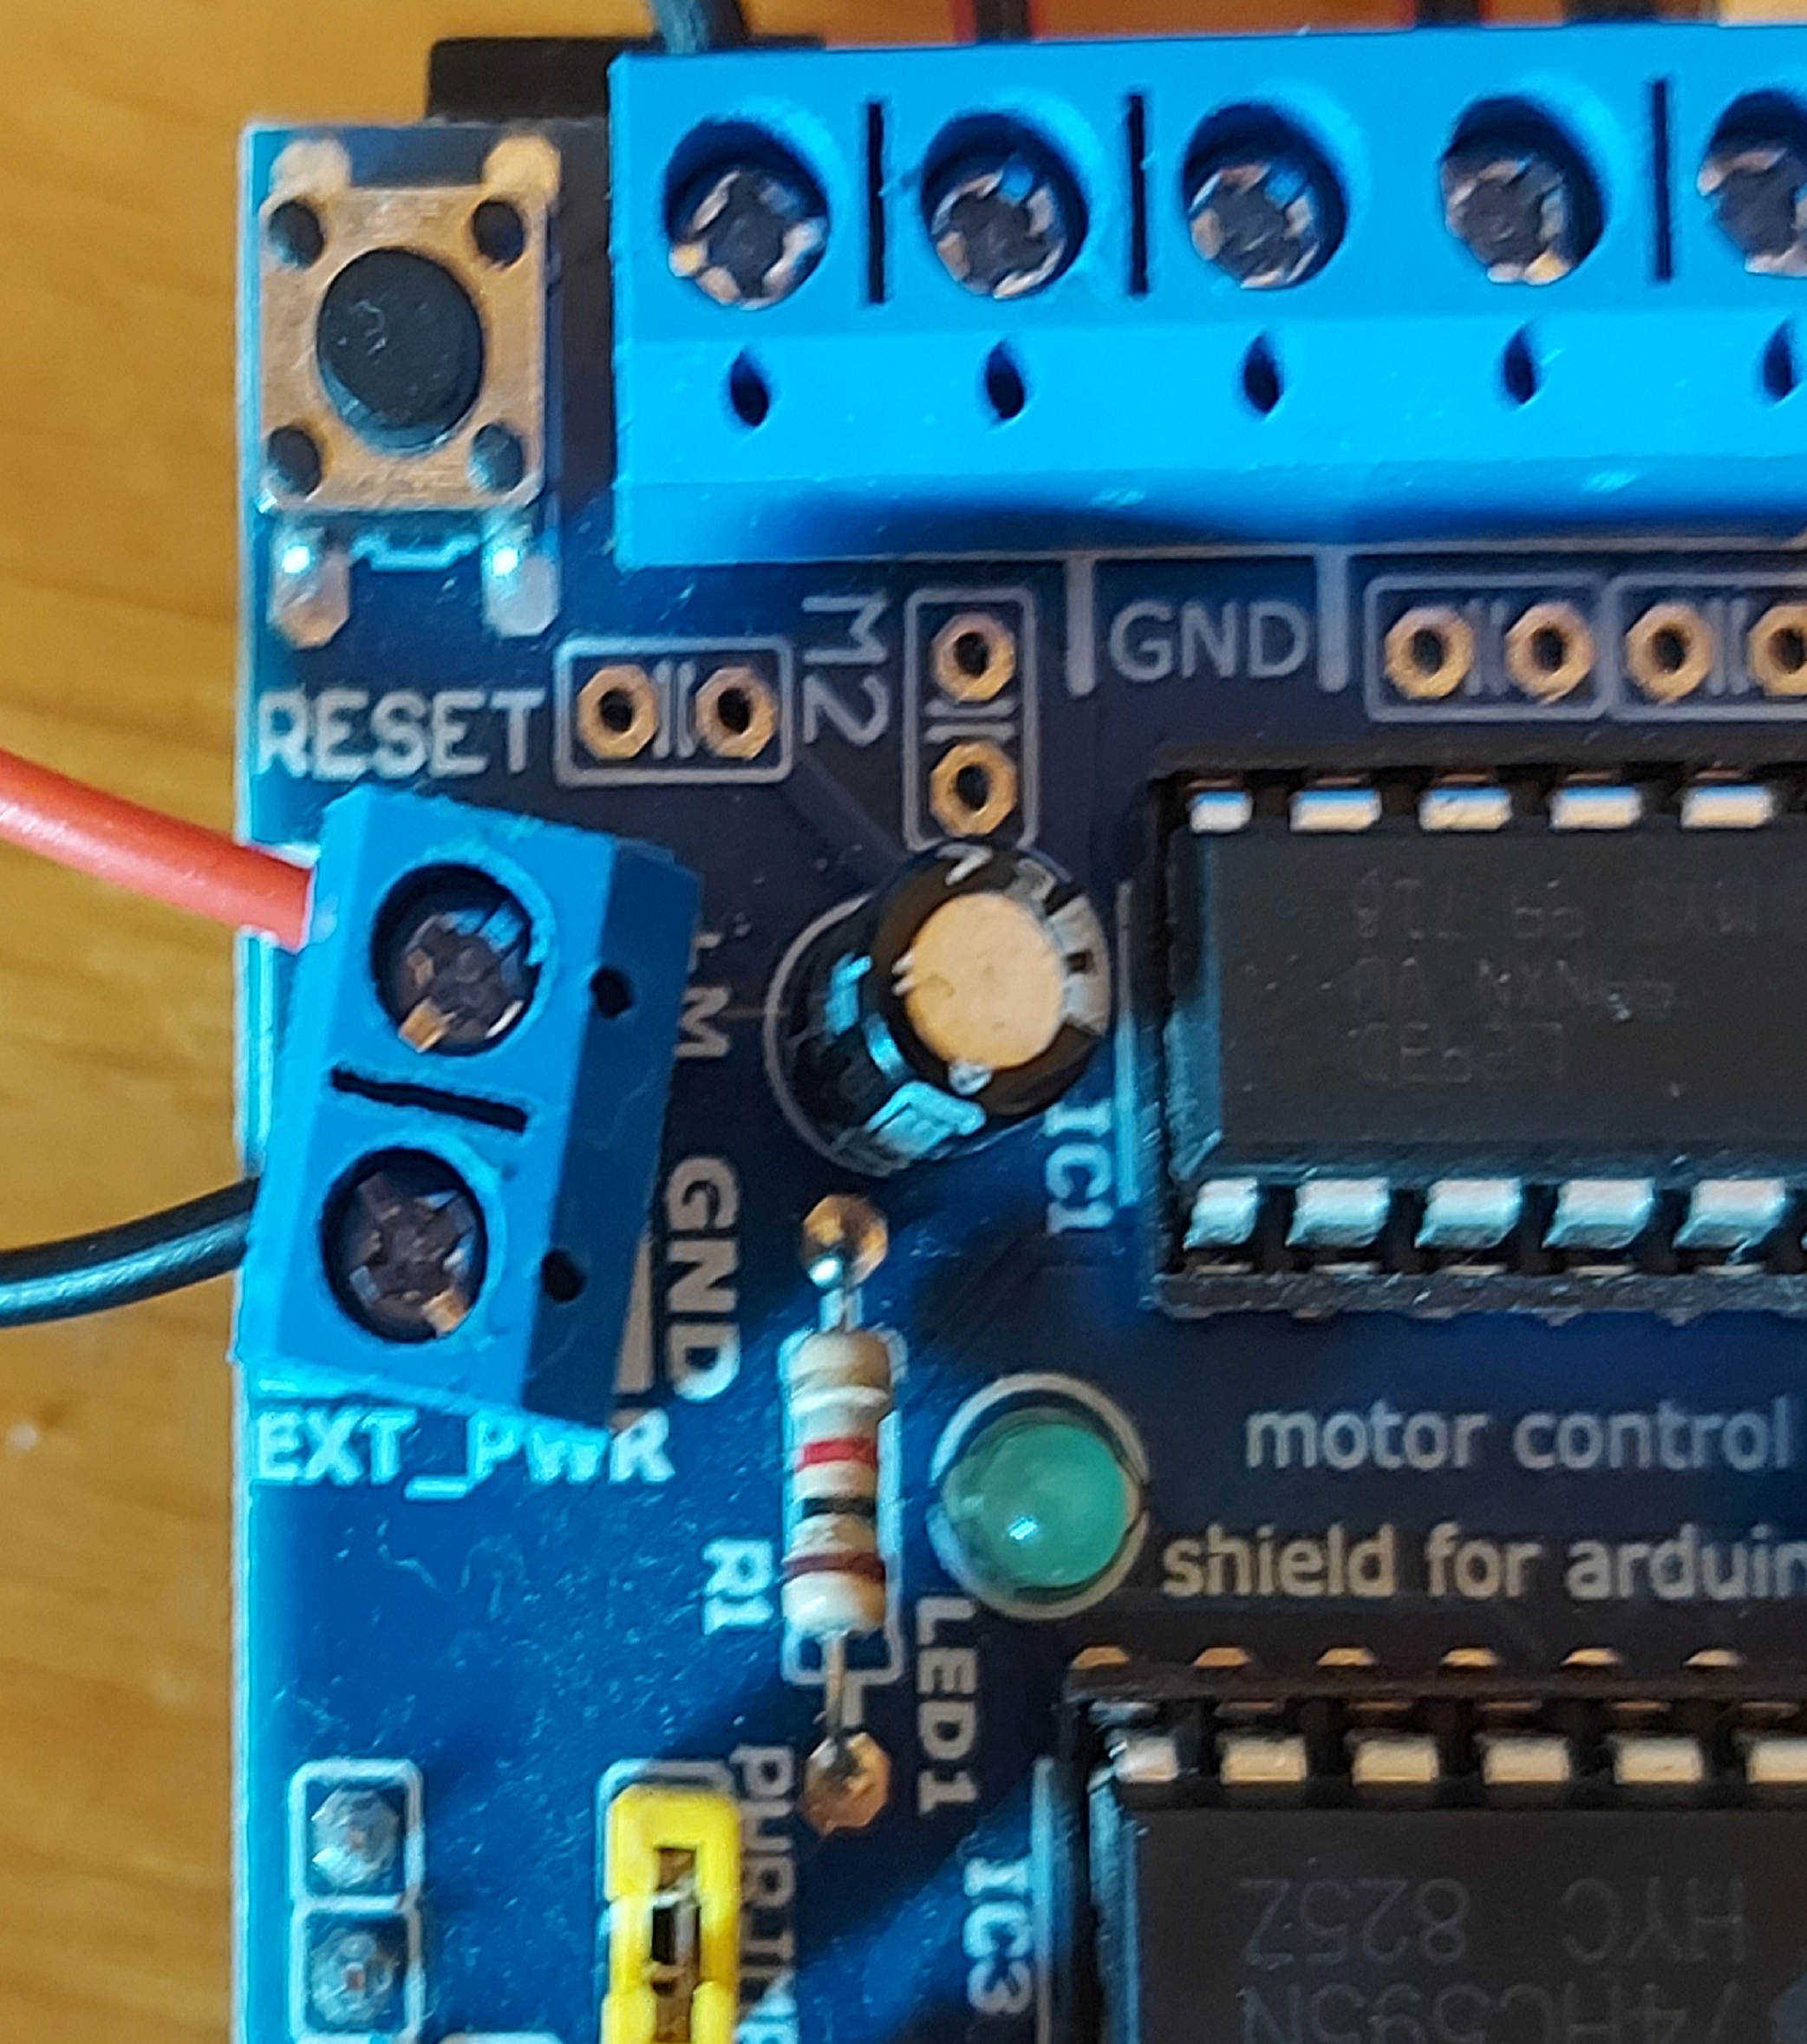
\includegraphics[width=5cm]{images/robot_build/akku-connect}
	\includegraphics[width=5cm]{images/robot_build/shieldre-bekotes}
	\caption{A shield-re való bekötés}
	\label{shieldre-bekotes}
\end{figure}

\subsection{Szenzorok felhelyezése}
Helyezzük fel a robot elejére a 2 db infravörös szenzort úgy, hogy a szenzorok között legalább 2-4 cm távolság legyen (a szenzorok közötti távolság méretét a követendő vonal vastagsága határozza meg), majd jumper kábel segítségével csatlakoztassuk ezeket a shield-en található A0 és A1-es, valamint az ehhez tartozó GND és VCC jelölésű portokhoz. (szemből nézve jobb oldali szenzor A0, bal oldali A1).

Ezek után helyezzük fel a szervó motort a szenzorok közé, majd erre a tartóelemet, a hozzá rögzített ultrahang szenzorral. Az ultrahang szenzor ’Trig’ és ’Echo’ jelzéssel ellátott tüskéit csatlakoztassuk a digitális 0 és 1 portokhoz, valamint GND és VCC tüskéit egy-egy GND és VCC porthoz. A szervó motor vezetékét csatlakoztassuk a shield-en található SERVO\_2 jelzésű tüskesorhoz.

A korábbi lépések elvégzése után helyezzük fel a Bluetooth modult, majd csatlakoztassuk a TX -- Transmitter és RX -- Receiver tüskéket a digitális 3 és 13 portokra, valamint a VCC és GND tüskéket a szenzorokhoz hasonlóan a shield VCC és GND tüskéihez.

\subsection{A program telepítése az alaplapra}
Csatlakoztassuk a mikrokontrollert a számítógéphez. Nyissuk meg a letöltött mappában található ’.ino’ kiterjesztésű fájlt az Arduino IDE segítségével. Az Eszközök -> Alaplap menüpontban válasszuk ki a használt alaplap típusát, valamint a portot amelyen keresztül csatlakoztattuk a számítógéphez. Kattintsunk a feltöltés gombra. 

Amint elkészül a feltöltés az IDE jelzi, ezek után az alaplapot leválaszthatjuk. A telepítés után helyezzük el a mikrokontrollert az alvázon és csatlakoztassuk hozzá a shield-et.

Utolsó lépésként a felhelyezett akkumulátor tartóba helyezzük el a 2 db 18650-es akkumulátort ügyelve a pólusok helyességére, majd a kapcsoló kapcsolásával lássuk el energiával az alaplapot, így elindítva a robotot.
\begin{figure}[h]
	\centering
	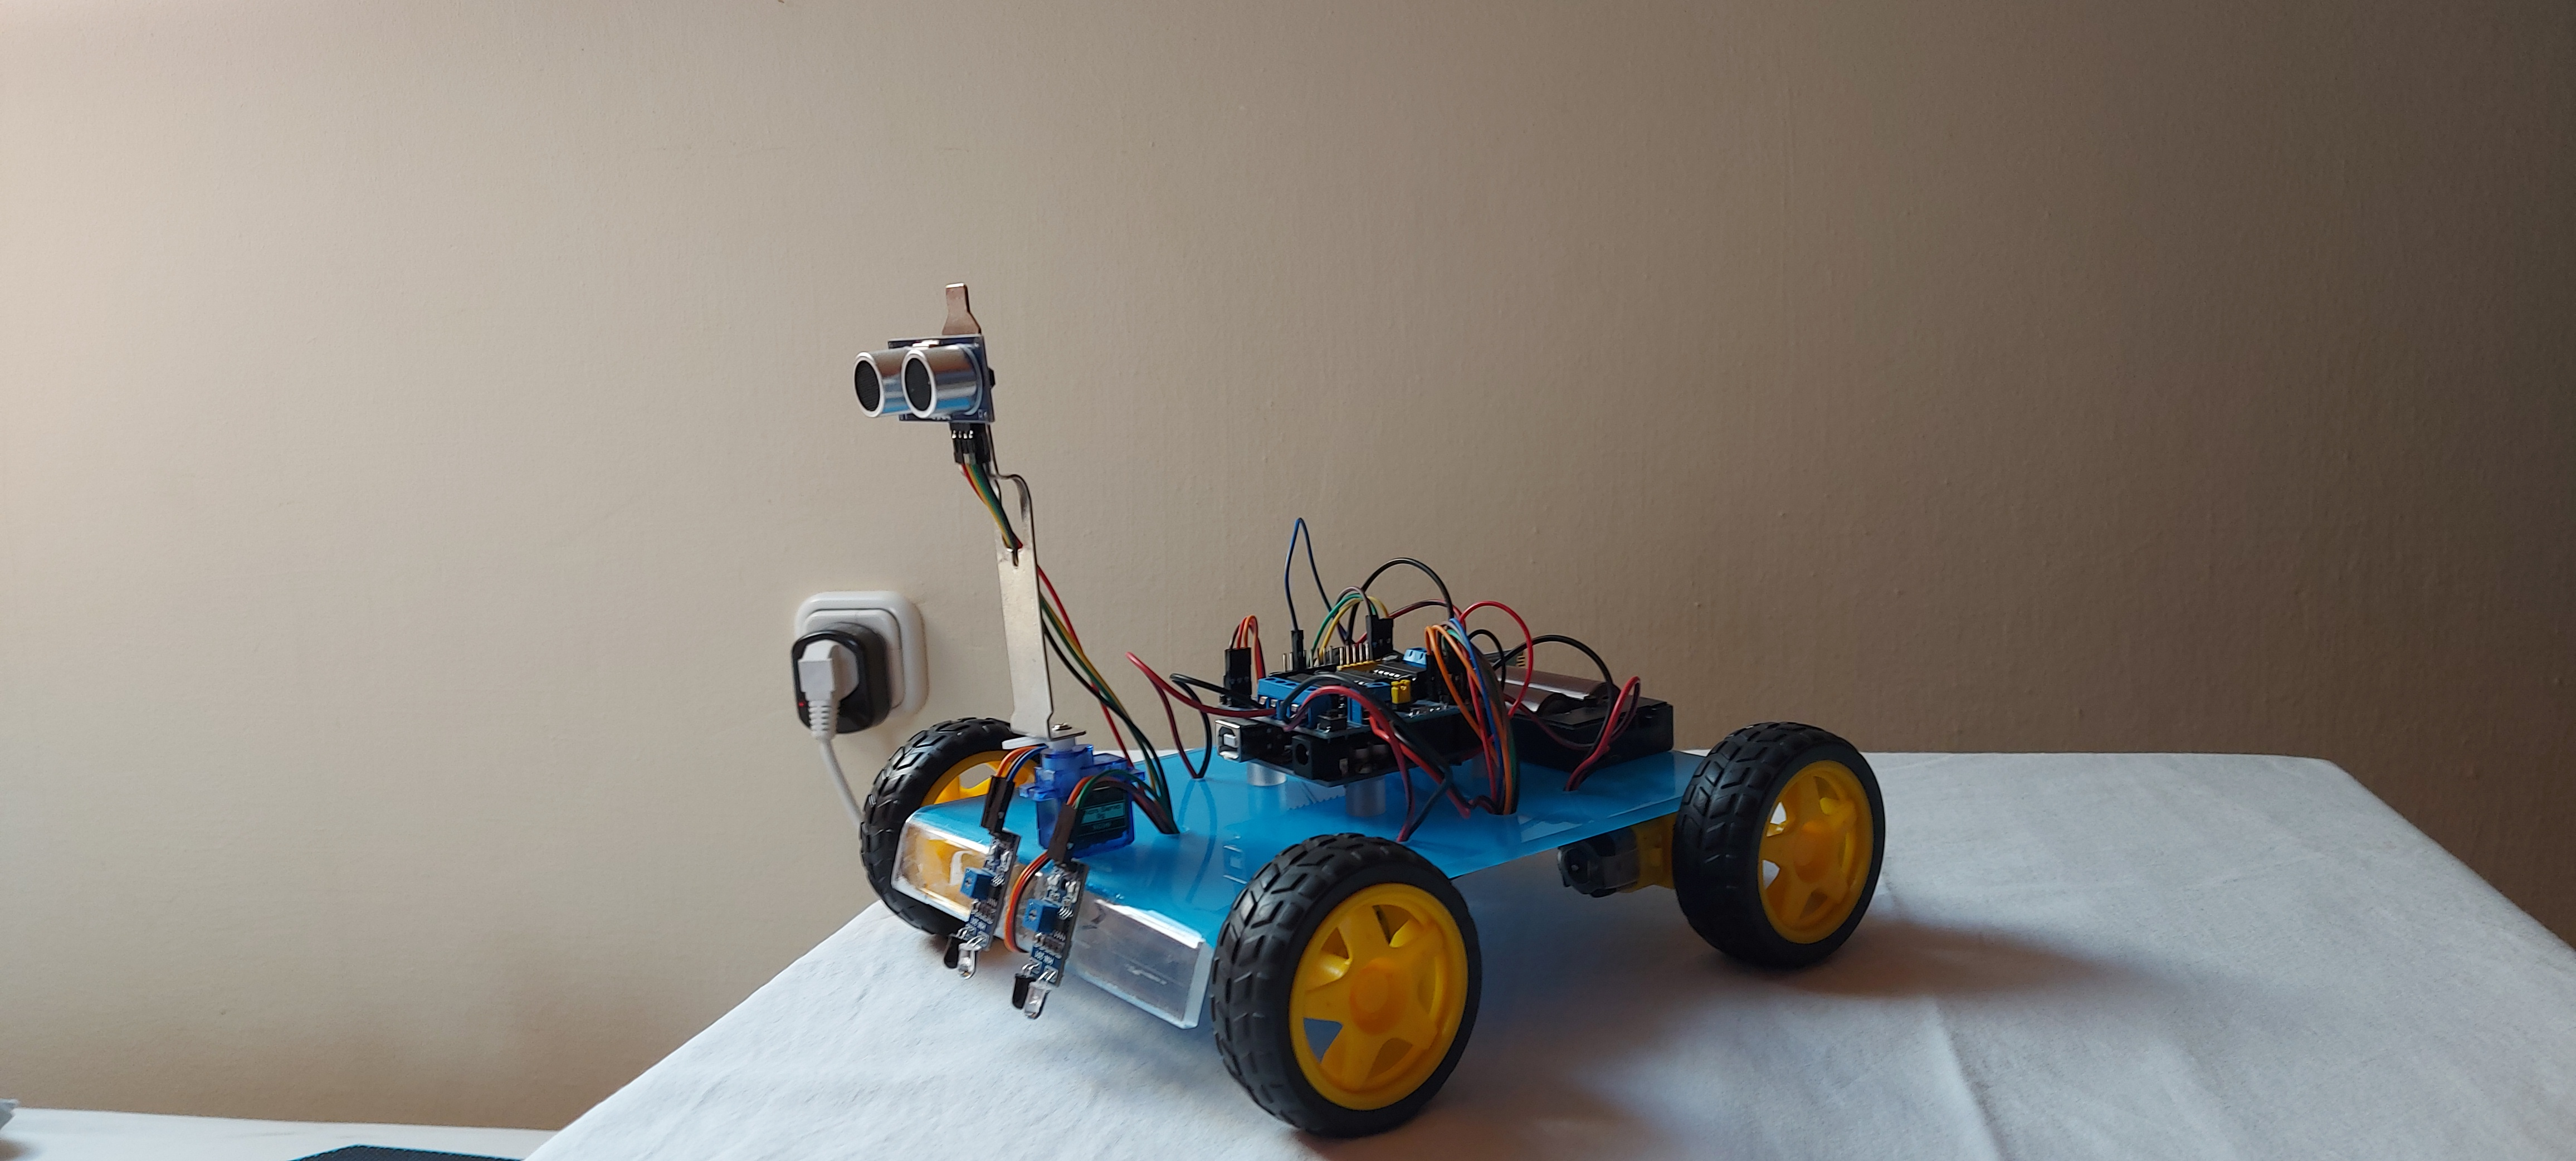
\includegraphics[width=\linewidth]{images/robot_build/finished_robot}
	\caption{A kész robot}
	\label{finished_robot}
\end{figure}
\section{A telefonon elvégzendő lépések}
Mielőtt a robotot vezérelni tudnánk el kell végeznünk néhány lépést.
\subsection{Az alkalmazás telepítése}
Mivel az alkalmazás még nem érhető el a PlayStore-on, ezért a telepítést manuálisan kell elvégeznünk. Ennek menete:
\begin{enumerate}
	\item A számítógépről másoljuk a készülékre az 'app-debug.apk' nevű fájlt
	\item Engedélyezzük a Beállításokban az ismeretlen forrásból származó alkalmazások telepítését
	\item Nyissuk meg a telefon fájlkezelő programját, majd keressük ki és futtassuk a fájlt.
	\item A megjelenő üzenetetnél válasszuk a 'Telepítés' lehetőséget
	\item Az installálás közben felugró 'PlayProtect' üzenetkor válasszuk a 'Telepítés mégis' opciót
	\item Amennyiben megkapjuk az 'Alkalmazás telepítve' üzenetet a telepítés sikeres volt, használhatjuk az alkalmazást
\end{enumerate}

Fontos megjegyezni, hogy a sikertelen telepítés főbb okai a következők lehetnek:
\begin{itemize}
	\item A telefon nem rendelkezik elegendő szabad tárhellyel
	\item Az alkalmazás nem kompatibilis a készülék Android verziójával
	\item Nem engedélyezett az ismeretlen forrásból származó alkalmazások telepítése
\end{itemize}
\subsection{Bluetooth párosítás}
Ahhoz, hogy a robothoz csatlakozni tudjunk először párosítani kell a készülékünket a roboton található HC-05 modullal. Ezt úgy tudjuk megtenni, hogy a telefonon elnavigálunk a Beállítások $\rightarrow$ Kapcsolatok $\rightarrow$ Bluetooth menüpontra, majd bekapcsoljuk a telefonban található Bluetooth egységet.

Ezek után a roboton bekapcsoljuk az akkumulátort, ezzel energiával látjuk el a HC-05-ös modult, ami ezt követően megjelenik az elérhető eszközök listájában.

A párosításhoz ki kell választanunk az eszközt és a felugró párbeszédablakban jelszónak az '1234' számsort kell beírnunk. Amint a párosítás megtörtént az applikációt indíthatjuk.
\subsection{Az alkalmazás első indítása}
Az alkalmazás indítását követően a kezdőképernyő fogad minket (lásd \ref{home-screen}~ábra).Itt az ,,Eszközök'' gomb megnyomása után láthatóvá válik a párosított eszközök listája.

Miután kiválasztottuk a HC-05-ös szenzort a listából a ,,Követés'', ,,Irányítás'' és ,,Log'' gombok valamelyikét megnyomva a telefon csatlakozik a robothoz.

Amennyiben a ,,Log'' gombot választjuk az applikáció a Naplózási képernyőre navigál minket, ahol az első futtatás alkalmával engedélyt kell adnunk az applikációnak a tárhely eléréséhez. Ha ezt nem tesszük meg a Naplófájlt nem fogjuk tudni menteni mindaddig, amíg az engedélyt meg nem adjuk. Az engedély megadása után az applikáció összes funkciója használható.
\begin{figure}[h]
	\centering
	\includegraphics[width=\columnwidth]{images/app_screen/permission_grant}
	\caption{Engedélyadás}
	\label{grant_permission}
\end{figure}
\chapter{Összegzés és továbbfejlesztés}\label{fejezet_8}
\emph{,,Always code as if the guy who ends up maintaining your code will be a violent psychopath who knows where you live'' -- John Woods}
\section{Összegzés}
A projekt jelenlegi állapotában a \ref{vágyálom}~fejezetben megfogalmazottaknak eleget tettem, vagyis a robot képes egy előre megadott pálya követésére, a követés közben észlelt akadály(ok) kikerülésére és a pálya újbóli megtalálására. A robot továbbá irányítható egy telefonnal, valamint a telefonon keresztül el tudjuk érni a robot által vezetett naplófájlt és ezt a telefonra menthetjük.

A végtermékkel sikerült egy olyan könnyen módosítható projektet megvalósítanom, mely különböző életkorú és programozási tapasztalattal rendelkező diákok oktatására és ismereteik bővítésére is alkalmas, valamint hobbi felhasználók részére sem bonyolult.

Bár a végtermék teljes, szoftveres és hardveres fejlesztés is lehetséges, a továbbiakban ezekről olvashatunk.
\section{Hardverre vonatkozó fejlesztés}
Ahogy \az{\ref{jelenlegi_helyzet}~fejezetben} is olvasható az éles kanyarok alkalmanként hibásan kerülnek bevételre. Ennek megoldását nyújthatja, ha a vonal érzékelésére másfajta szenzort használunk (pl.: digitális vonalkövető szenzor), mely pontosabban képes érzékelni a pálya vonalában végbemenő változást.
Lehetséges megoldási módszer a motorok más formában való kezelése az IR szenzorról kapott jelzéskor (nagyobb nyomaték azokra a motorokra melyeknek előre kell mozdulni).

További hardver fejlesztés lehet egy kamera beépítése a robot elejére és ezt felhasználva az irányításért felelős okostelefonon élő képet kaphatunk arról, hogy a robot éppen merre jár. Ennek segítségével a telefonnal való irányításkor nincs szükség arra, hogy a robotot ténylegesen lássuk, hanem a kamera képére hivatkozva ki tudjuk kerülni az akadályokat, valamint egy jobb felhasználói élményt biztosít. Ehhez szükséges egy olyan telefon, amely kellő hardverrel rendelkezik egy ilyen program futtatásához, valamint a külső akkumulátor is gyorsabban fog merülni.
\section{Android szoftverre vonatkozó fejlesztés}
A szoftverben két nagy fejlesztési lehetőségre lettem figyelmes:
\begin{itemize}
	\item Logolás fejlesztése (hardver fejlesztése is szükséges)
	\item Súgó felület bővítése
\end{itemize}
Amennyiben beépítésre kerül a robotra egy giroszkóp meg lehet mondani, hogy az egyes kanyarok elvégzésekor a robot milyen szögben fordult jobbra/balra, illetve az is, hogy a felületben milyen változás történik (a robot emelkedőn halad felfele, vagy lejtőn lefele).

Ezeket az adatokat felhasználva el lehet készíteni egy statisztikát, valamint automata követéskor a kanyarodások közötti időeltérés és a kanyarok szögének ismeretében a pálya vizualizálása is lehetségessé válhat.

További fejlesztési lehetőség a felhasználói útmutató implementálása az alkalmazás Súgó felületére, ugyanis ha a felhasználó nincs birtokában az említett dokumentumnak (\ref{fejezet_7}.~fejezet) a robot összeszerelésekor nem tudhatja, hogy az adott szenzort/motort hova kell csatlakoztatnia..
\section{A hardver biztosítására vonatkozó fejlesztés}
A projekt jelenlegi állapotában fedetlenül található meg az összes szenzor, kábel, motor és a mikrokontroller is, ezért fennáll az esélye annak, hogy valamely komponens megsérül, ezzel meggátolva a robot megfelelő működését.

A komponensek biztosítására lehetséges egy olyan váz megtervezése és 3D nyomtatása, mely védelmet biztosít a hardver elemeinek, illetve így egy olyan kinézetet lehet adni a robotnak, amilyet a felhasználó elképzel.
\begin{thebibliography}{1}
	\bibitem{Arduino} \textsc{Harsányi Réka -- Juhász Márton András: Fizikai számítástechnika: elektronikai alapok és Arduino programozás}
	\bibitem{CPP} \textsc{Lapteva Natalia -- Tóth Bertalan: Programozzunk C++ nyelven}
	\bibitem{Java} \textsc{Nagy Gusztáv -- Java programozás}
	\bibitem{Android}	\textsc{Fehér Krisztián: Alkalmazásfejlesztés Android Stúdió rendszerben}
	\bibitem{Arduino IDE} \textsc{\url{https://www.arduino.cc/en/Guide/Environment}}
	\bibitem{NAT} \textsc{\url{https://www.oktatas.hu/kozneveles/kerettantervek/2020\_nat}}
	\bibitem{Ultrahang_Szenzor}
	\textsc{\url{https://create.arduino.cc/projecthub/abdularbi17/ultrasonic-sensor-hc-sr04-with-arduino-tutorial-327ff6}}
	\bibitem{Bluetooth_active}
	\textsc{\url{https://stackoverflow.com/questions/7672334/how-to-check-if-bluetooth-is-enabled-programmatically}}
	\bibitem{Bluetooth_enable}
	\textsc{\url{https://stackoverflow.com/questions/3806536/how-to-enable-disable-bluetooth-programmatically-in-android}}
	\bibitem{Bluetooth_connect}
	\textsc{\url{https://stackoverflow.com/questions/5171248/programmatically-connect-to-paired-bluetooth-device}}
	\bibitem{Data_Recieve}
	\textsc{\url{https://stackoverflow.com/questions/45140098/how-to-send-receive-messages-via-bluetooth-android-studio}}
\end{thebibliography}
\end{document}